\documentclass[,aspectratio=43]{beamer}

\usepackage{empheq}


% Load theme ---------------------------------------------------------------------------------

\usetheme[progressdots,transitions,banner,logo]{ubd}

\newcommand{\prevarblock}{%
 \setbeamercolor{block title}{fg=lightcyan!50,bg=myrtlegreen}
 \setbeamercolor{block body}{parent=normal text,bg=lightcyan!50,fg=myrtlegreen}
}
\newenvironment{varblock}[1]{%
  \prevarblock
  \begin{block}{#1}}{\end{block}}

% Information for the title page -------------------------------------------------------------
\author{Haziq Jamil}

\title{An Interactive Introduction to \LaTeX}

\subtitle{TLC Workshop}

\institute{Mathematical Sciences, Faculty of Science, UBD\\
\url{https://haziqj.ml}}

\date{Wednesday, 23 November 2022}

% Font fix -----------------------------------------------------------------------------------
% \usepackage{ifxetex,ifluatex}
% \ifnum 0\ifxetex 1\fi\ifluatex 1\fi=0 % if pdftex
%   \usepackage[T1]{fontenc}
%   \usepackage[utf8]{inputenc}
%   \usepackage{textcomp} % provide euro and other symbols
% \else % if luatex or xetex
%   \usepackage{unicode-math}
%   \defaultfontfeatures{Scale=MatchLowercase}
%   \defaultfontfeatures[\rmfamily]{Ligatures=TeX,Scale=1}
% \fi

\usepackage{soul}
\makeatletter
\let\HL\hl
\renewcommand\hl{%
  \let\set@color\beamerorig@set@color
  \let\reset@color\beamerorig@reset@color
  \HL}
\makeatother
% https://tex.stackexchange.com/questions/460731/highlight-color-a-part-of-text-in-block-in-beamer
\newcommand{\hlc}[2][yellow]{{%
    \colorlet{foo}{#1}%
    \sethlcolor{foo}\hl{#2}}%
}
% https://tex.stackexchange.com/questions/352956/how-to-highlight-text-with-an-arbitrary-color

% knitr stuff --------------------------------------------------------------------------------
\usepackage{color}
\usepackage{fancyvrb}
\newcommand{\VerbBar}{|}
\newcommand{\VERB}{\Verb[commandchars=\\\{\}]}
\DefineVerbatimEnvironment{Highlighting}{Verbatim}{commandchars=\\\{\}}
% Add ',fontsize=\small' for more characters per line
\usepackage{framed}
\definecolor{shadecolor}{RGB}{248,248,248}
\newenvironment{Shaded}{\begin{snugshade}}{\end{snugshade}}
\newcommand{\AlertTok}[1]{\textcolor[rgb]{0.94,0.16,0.16}{#1}}
\newcommand{\AnnotationTok}[1]{\textcolor[rgb]{0.56,0.35,0.01}{\textbf{\textit{#1}}}}
\newcommand{\AttributeTok}[1]{\textcolor[rgb]{0.77,0.63,0.00}{#1}}
\newcommand{\BaseNTok}[1]{\textcolor[rgb]{0.00,0.00,0.81}{#1}}
\newcommand{\BuiltInTok}[1]{#1}
\newcommand{\CharTok}[1]{\textcolor[rgb]{0.31,0.60,0.02}{#1}}
\newcommand{\CommentTok}[1]{\textcolor[rgb]{0.56,0.35,0.01}{\textit{#1}}}
\newcommand{\CommentVarTok}[1]{\textcolor[rgb]{0.56,0.35,0.01}{\textbf{\textit{#1}}}}
\newcommand{\ConstantTok}[1]{\textcolor[rgb]{0.00,0.00,0.00}{#1}}
\newcommand{\ControlFlowTok}[1]{\textcolor[rgb]{0.13,0.29,0.53}{\textbf{#1}}}
\newcommand{\DataTypeTok}[1]{\textcolor[rgb]{0.13,0.29,0.53}{#1}}
\newcommand{\DecValTok}[1]{\textcolor[rgb]{0.00,0.00,0.81}{#1}}
\newcommand{\DocumentationTok}[1]{\textcolor[rgb]{0.56,0.35,0.01}{\textbf{\textit{#1}}}}
\newcommand{\ErrorTok}[1]{\textcolor[rgb]{0.64,0.00,0.00}{\textbf{#1}}}
\newcommand{\ExtensionTok}[1]{#1}
\newcommand{\FloatTok}[1]{\textcolor[rgb]{0.00,0.00,0.81}{#1}}
\newcommand{\FunctionTok}[1]{\textcolor[rgb]{0.00,0.00,0.00}{#1}}
\newcommand{\ImportTok}[1]{#1}
\newcommand{\InformationTok}[1]{\textcolor[rgb]{0.56,0.35,0.01}{\textbf{\textit{#1}}}}
\newcommand{\KeywordTok}[1]{\textcolor[rgb]{0.13,0.29,0.53}{\textbf{#1}}}
\newcommand{\NormalTok}[1]{#1}
\newcommand{\OperatorTok}[1]{\textcolor[rgb]{0.81,0.36,0.00}{\textbf{#1}}}
\newcommand{\OtherTok}[1]{\textcolor[rgb]{0.56,0.35,0.01}{#1}}
\newcommand{\PreprocessorTok}[1]{\textcolor[rgb]{0.56,0.35,0.01}{\textit{#1}}}
\newcommand{\RegionMarkerTok}[1]{#1}
\newcommand{\SpecialCharTok}[1]{\textcolor[rgb]{0.00,0.00,0.00}{#1}}
\newcommand{\SpecialStringTok}[1]{\textcolor[rgb]{0.31,0.60,0.02}{#1}}
\newcommand{\StringTok}[1]{\textcolor[rgb]{0.31,0.60,0.02}{#1}}
\newcommand{\VariableTok}[1]{\textcolor[rgb]{0.00,0.00,0.00}{#1}}
\newcommand{\VerbatimStringTok}[1]{\textcolor[rgb]{0.31,0.60,0.02}{#1}}
\newcommand{\WarningTok}[1]{\textcolor[rgb]{0.56,0.35,0.01}{\textbf{\textit{#1}}}}
\usepackage{graphicx,grffile}
\makeatletter
\def\maxwidth{\ifdim\Gin@nat@width>\linewidth\linewidth\else\Gin@nat@width\fi}
\def\maxheight{\ifdim\Gin@nat@height>\textheight\textheight\else\Gin@nat@height\fi}
\makeatother
% Scale images if necessary, so that they will not overflow the page
% margins by default, and it is still possible to overwrite the defaults
% using explicit options in \includegraphics[width, height, ...]{}
\setkeys{Gin}{width=\maxwidth,height=\maxheight,keepaspectratio}
% Set default figure placement to htbp
\makeatletter
\def\fps@figure{htbp}
\makeatother
\setlength{\emergencystretch}{3em} % prevent overfull lines
\providecommand{\tightlist}{%
  \setlength{\itemsep}{0pt}\setlength{\parskip}{0pt}}
\setcounter{secnumdepth}{-\maxdimen} % remove section numbering

% Packages -----------------------------------------------------------------------------------
% \setlength{\parskip}{1em}
\usepackage{tikz}
\usetikzlibrary{shapes.geometric,fit,arrows.meta}
\usepackage{xltabular}
\usepackage{longtable,booktabs,multirow,colortbl}
\usepackage{multicol}
\usepackage{caption}
% Make caption package work with longtable
\makeatletter
\def\fnum@table{\tablename~\thetable}
\makeatother
\usepackage{lipsum}
\usepackage{csquotes}

% To use arabic -----------------------------------------------------------------------------
% WARNING: Using arabic script causes some issues with footnotes.
% Packages are not loaded by default

\usepackage{polyglossia}  
\setdefaultlanguage{english}
\setotherlanguage{arabic} % to use arabic
\newfontfamily\arabicfontsf[Script=Arabic]{Amiri}
\usepackage{xeCJK}
\setCJKmainfont{SimSun}
% \usepackage{fontspec}


% % Fix for footnotes not showing when arabic script used
% % https://tex.stackexchange.com/questions/228075/beamer-in-arabic-language-doesnt-accept-footnotes
% \makeatletter
% \let\@footnotetext=\beamer@framefootnotetext
% \makeatother

% % Fix for footnotes not showing when using \footnote<.->
% \let\oldfootnote\footnote
% \renewcommand{\footnote}{\only<+->\oldfootnote}
% % https://stackoverflow.com/questions/62345074/show-footnote-only-after-a-pause-in-beamer-with-r-markdown

% Fonts -----------------------------------------------------------------------------------
\usepackage{cmbright}
\usefonttheme{default}
\usepackage{pifont}% http://ctan.org/pkg/pifont
\newcommand{\cmark}{\ding{51}}%
\newcommand{\xmark}{\ding{55}}%

% Bibliography
\usepackage[style=numeric,giveninits=true,maxcitenames=2,maxbibnames=99,backend=biber,natbib]{biblatex}
\addbibresource{refs.bib}

% Fix URL, DOI, ISBN, etc. font in biblatex
% https://tex.stackexchange.com/questions/416093/change-font-of-the-word-url-before-the-actual-url-in-biblatex
% \renewcommand*{\mkbibacro}[1]{#1}  

\newcommand{\thankyou}{%
	{
		\begin{frame}[plain,noframenumbering]{End}
			\centering
			\Huge Thank you!
		\end{frame}
	}

}

% Maths -----------------------------------------------
\newcommand*\mybox[1]{%
\colorbox{navyblue!35}{#1}}

\usepackage[skins,theorems]{tcolorbox}
\tcbset{highlight math style={enhanced,
  colframe=navyblue,colback=white,arc=2pt,boxrule=1pt}}

\usepackage{amssymb}
\usepackage{dsfont}  % for indicator variables \mathsds{1}
\usepackage{bm}  % for better bold script
\usepackage[makeroom]{cancel}
\usepackage{centernot}
\renewcommand{\CancelColor}{\color{gray}}
\newcommand{\bzero}{{\bm 0}}
\newcommand{\bone}{{\bm 1}}
%\newcommand{\ba}{{\bm a}}
\newcommand{\bb}{{\bm b}}
\newcommand{\bc}{{\bm c}}
\newcommand{\bd}{{\bm d}}
\newcommand{\be}{{\bm e}}
\newcommand{\bff}{{\bm f}}
\newcommand{\bg}{{\bm g}}
\newcommand{\bh}{{\bm h}}
\newcommand{\bi}{{\bm i}}
\newcommand{\bj}{{\bm j}}
\newcommand{\bk}{{\bm k}}
\newcommand{\bl}{{\bm l}}
\newcommand{\bmm}{{\bm m}}
\newcommand{\bn}{{\bm n}}
\newcommand{\bo}{{\bm o}}
\newcommand{\bp}{{\bm p}}
\newcommand{\bq}{{\bm q}}
\newcommand{\br}{{\bm r}}
\newcommand{\bs}{{\bm s}}
\newcommand{\bt}{{\bm t}}
\newcommand{\bu}{{\bm u}}
\newcommand{\bv}{{\bm v}}
\newcommand{\bw}{{\bm w}}
\newcommand{\bx}{{\bm x}}
\newcommand{\by}{{\bm y}}
\newcommand{\bz}{{\bm z}}
\newcommand{\bA}{{\bm A}}
\newcommand{\bB}{{\bm B}}
\newcommand{\bC}{{\bm C}}
\newcommand{\bD}{{\bm D}}
\newcommand{\bE}{{\bm E}}
\newcommand{\bF}{{\bm F}}
\newcommand{\bG}{{\bm G}}
\newcommand{\bH}{{\bm H}}
\newcommand{\bI}{{\bm I}}
\newcommand{\bJ}{{\bm J}}
\newcommand{\bK}{{\bm K}}
\newcommand{\bL}{{\bm L}}
\newcommand{\bM}{{\bm M}}
\newcommand{\bN}{{\bm N}}
\newcommand{\bO}{{\bm O}}
\newcommand{\bP}{{\bm P}}
\newcommand{\bQ}{{\bm Q}}
\newcommand{\bR}{{\bm R}}
\newcommand{\bS}{{\bm S}}
\newcommand{\bT}{{\bm T}}
\newcommand{\bU}{{\bm U}}
\newcommand{\bV}{{\bm V}}
\newcommand{\bW}{{\bm W}}
\newcommand{\bX}{{\bm X}}
\newcommand{\bY}{{\bm Y}}
\newcommand{\bZ}{{\bm Z}}

% Greek bold letters
\newcommand{\balpha}{{\bm\alpha}}
\newcommand{\bbeta}{{\bm\beta}}
\newcommand{\bgamma}{{\bm\gamma}}
\newcommand{\bdelta}{{\bm\delta}}
\newcommand{\bepsilon}{{\bm\epsilon}}
\newcommand{\bvarepsilon}{{\bm\varepsilon}}
\newcommand{\bzeta}{{\bm\zeta}}
\newcommand{\bfeta}{{\bm\eta}}
\newcommand{\boldeta}{{\bm\eta}}
\newcommand{\btheta}{{\bm\theta}}
\newcommand{\bvartheta}{{\bm\vartheta}}
\newcommand{\biota}{{\bm\iota}}
\newcommand{\bkappa}{{\bm\kappa}}
\newcommand{\blambda}{{\bm\lambda}}
\newcommand{\bmu}{{\bm\mu}}
\newcommand{\bnu}{{\bm\nu}}
\newcommand{\bxi}{{\bm\xi}}
\newcommand{\bpi}{{\bm\pi}}
\newcommand{\bvarpi}{{\bm\varpi}}
\newcommand{\brho}{{\bm\rho}}
\newcommand{\bvarrho}{{\bm\varrho}}
\newcommand{\bsigma}{{\bm\sigma}}
\newcommand{\bvarsigma}{{\bm\varsigma}}
\newcommand{\btau}{{\bm\tau}}
\newcommand{\bupsilon}{{\bm\upsilon}}
\newcommand{\bphi}{{\bm\phi}}
\newcommand{\bvarphi}{{\bm\varphi}}
\newcommand{\bchi}{{\bm\chi}}
\newcommand{\bpsi}{{\bm\psi}}
\newcommand{\bomega}{{\bm\omega}}

\newcommand{\bGamma}{{\bm\Gamma}}
\newcommand{\bDelta}{{\bm\Delta}}
\newcommand{\bTheta}{{\bm\Theta}}
\newcommand{\bLambda}{{\bm\Lambda}}
\newcommand{\bXi}{{\bm\Xi}}
\newcommand{\bPi}{{\bm\Pi}}
\newcommand{\bSigma}{{\bm\Sigma}}
\newcommand{\bUpsilon}{{\bm\Upsilon}}
\newcommand{\bPhi}{{\bm\Phi}}
\newcommand{\bPsi}{{\bm\Psi}}
\newcommand{\bOmega}{{\bm\Omega}}

% Probability and Statistics
\DeclareMathOperator{\Prob}{P}
\DeclareMathOperator{\E}{E}
\DeclareMathOperator{\Var}{Var}
\DeclareMathOperator{\Cov}{Cov}
\DeclareMathOperator{\Corr}{Corr}
\DeclareMathOperator{\sd}{sd}
\DeclareMathOperator{\se}{se}
\DeclareMathOperator{\N}{N}
\DeclareMathOperator{\Bin}{Bin}
\DeclareMathOperator{\Bern}{Bern}
\DeclareMathOperator{\Dir}{Dir}
\DeclareMathOperator{\Wis}{Wis}
\DeclareMathOperator{\logit}{logit}
\DeclareMathOperator{\expit}{expit}
\DeclareMathOperator{\Mult}{Mult}
\DeclareMathOperator{\Cat}{Cat}
\DeclareMathOperator{\Pois}{Poi}
\DeclareMathOperator{\Geom}{Geom}
\DeclareMathOperator{\NBin}{NBin}
\DeclareMathOperator{\Exp}{Exp}
\DeclareMathOperator{\Betadist}{Beta}
\DeclareMathOperator{\Hypergeom}{Hypergeom}
\DeclareMathOperator{\Cauchy}{Cauchy}
\DeclareMathOperator{\hCauchy}{half-Cauchy}
\DeclareMathOperator{\LKJ}{LKJ}
\DeclareMathOperator{\Unif}{Unif}
\DeclareMathOperator{\KL}{KL}
\DeclareMathOperator{\ind}{\mathds{1}}
\newcommand{\iid}{\,\overset{\text{iid}}{\sim}\,}
\DeclareMathOperator*{\plim}{plim}
\DeclareMathOperator{\Lik}{L}
\DeclareMathOperator{\Leb}{Leb}


% Blackboard bold
\newcommand{\bbR}{\mathbb{R}}
\newcommand{\bbN}{\mathbb{N}}
\newcommand{\bbZ}{\mathbb{Z}}
\newcommand{\bbC}{\mathbb{C}}
\newcommand{\bbS}{\mathbb{S}}
\newcommand{\bbH}{\mathbb{H}}
\newcommand{\bbP}{\mathbb{P}}
\newcommand{\bbQ}{\mathbb{Q}}
\newcommand{\bbE}{\mathbb{E}}

% Math calligraphic fonts
\newcommand{\cA}{{\mathcal A}}
\newcommand{\cB}{{\mathcal B}}
\newcommand{\cC}{{\mathcal C}}
\newcommand{\cD}{{\mathcal D}}
\newcommand{\cE}{{\mathcal E}}
\newcommand{\cF}{{\mathcal F}}
\newcommand{\cG}{{\mathcal G}}
\newcommand{\cH}{{\mathcal H}}
\newcommand{\cI}{{\mathcal I}}
\newcommand{\cJ}{{\mathcal J}}
\newcommand{\cK}{{\mathcal K}}
\newcommand{\cL}{{\mathcal L}}
\newcommand{\cM}{{\mathcal M}}
\newcommand{\cN}{{\mathcal N}}
\newcommand{\cO}{{\mathcal O}}
\newcommand{\cP}{{\mathcal P}}
\newcommand{\cQ}{{\mathcal Q}}
\newcommand{\cR}{{\mathcal R}}
\newcommand{\cS}{{\mathcal S}}
\newcommand{\cT}{{\mathcal T}}
\newcommand{\cU}{{\mathcal U}}
\newcommand{\cV}{{\mathcal V}}
\newcommand{\cW}{{\mathcal W}}
\newcommand{\cX}{{\mathcal X}}
\newcommand{\cY}{{\mathcal Y}}
\newcommand{\cZ}{{\mathcal Z}}


% Overbrace and underbrace
\newcommand{\myoverbrace}[3][gray!70]{{\color{#1}\overbrace{\color{black}#2}^{#3}}}
\newcommand{\myunderbrace}[3][gray!70]{{\color{#1}\underbrace{\color{black}#2}_{#3}}}


% Conveniences
\newcommand{\const}{\text{const.}}
\newcommand{\half}[1][1]{\frac{#1}{2}}  % \half for 1/2 or \half[n] for n/2, etc.
\DeclareMathOperator{\diag}{diag}
\DeclareMathOperator{\tr}{tr}
\DeclareMathOperator*{\argmin}{arg\,min}
\DeclareMathOperator*{\argmax}{arg\,max}

% Comments grey text
\newcommand{\mycomment}[2][10pt]{\hspace{#1}\rlap{\color{gray}\text{#2}}}

% Derivatives and integration
\let\d\relax
\DeclareMathOperator{\dd}{d}
\newcommand{\dint}{\dd\hspace{0.5pt}\!}
\newcommand{\d}{\text{d}}

% https://tex.stackexchange.com/questions/19981/how-to-write-rudins-symbol-for-absolute-continuity-of-measures
\DeclareFontFamily{U}{matha}{\hyphenchar\font45}
\DeclareFontShape{U}{matha}{m}{n}{
  <-6> matha5 <6-7> matha6 <7-8> matha7
  <8-9> matha8 <9-10> matha9
  <10-12> matha10 <12-> matha12
  }{}
% \DeclareFontShape{U}{matha}{m}{n}{
%   <5> <6> <7> <8> <9> <10> gen * matha
%   <10.95> matha10 <12> <14.4> <17.28>
%   <20.74> <24.88> matha12
%   }{}

\DeclareSymbolFont{matha}{U}{matha}{m}{n}
\DeclareMathSymbol{\Lt}{3}{matha}{"CE}

\graphicspath{ {figure/} }


\setbeamertemplate{itemize item}[circ]
\setbeamertemplate{itemize subitem}[circ]
\setbeamertemplate{itemize subsubitem}[circ]

\newenvironment{onlyhandout}{\only<handout>{}{}}



\usepackage{chemfig}
\setchemfig{atom sep = 2em, bond join = true}
\usepackage{chemmacros}
\chemsetup{modules = {all}}
\setbeamertemplate{caption}[numbered]



\begin{document}

\begin{frame}[plain,noframenumbering]
	\titlepage
\end{frame}

\begin{frame}[allowframebreaks=0.8]{Overview}
    \begin{multicols}{2}
  \tableofcontents
  \end{multicols}
  \end{frame}


\hypertarget{hello-world}{%
\section{Hello World}\label{hello-world}}

\begin{frame}{Why \LaTeX?}
\protect\hypertarget{why}{}
\begin{itemize}
\item
  It makes beautiful documents
\item
  Open source and active community. Lots of packages available.
\item
  Extensible document types (articles, presentation slides, books,
  theses, exam papers, etc.)
\end{itemize}
\end{frame}

\begin{frame}[fragile]{How does it work?}
\protect\hypertarget{how-does-it-work}{}
\begin{itemize}
\item
  You write your document in \texttt{plain\ text} with commands that
  describe its structure and meaning.
\item
  The \LaTeX program then processes your text and commands to produce a
  beautifully formatted document.
\end{itemize}

\begin{Shaded}
\begin{Highlighting}[]
\NormalTok{The rain in Spain falls }\FunctionTok{\textbackslash{}emph}\NormalTok{\{mainly\} on the plain.}
\end{Highlighting}
\end{Shaded}

\begin{center}
The rain in Spain falls \emph{mainly} on the plain.

\end{center}
\end{frame}

\begin{frame}[fragile]{More examples of commands and output\ldots{}}
\protect\hypertarget{more-examples-of-commands-and-output}{}
\begin{columns}[T]
\begin{column}{0.48\textwidth}
\begin{Shaded}
\begin{Highlighting}[]
\KeywordTok{\textbackslash{}begin}\NormalTok{\{}\ExtensionTok{itemize}\NormalTok{\}}
  \FunctionTok{\textbackslash{}item}\NormalTok{ Tea}
  \FunctionTok{\textbackslash{}item}\NormalTok{ Milk}
  \FunctionTok{\textbackslash{}item}\NormalTok{ Biscuits}
\KeywordTok{\textbackslash{}end}\NormalTok{\{}\ExtensionTok{itemize}\NormalTok{\}}
\end{Highlighting}
\end{Shaded}
\end{column}

\begin{column}{0.48\textwidth}
\vspace{2em}

\begin{itemize}
\item Tea
\item Milk
\item Biscuits
\end{itemize}
\end{column}
\end{columns}

\begin{columns}[T]
\begin{column}{0.48\textwidth}
\begin{Shaded}
\begin{Highlighting}[]
\KeywordTok{\textbackslash{}begin}\NormalTok{\{}\ExtensionTok{figure}\NormalTok{\}}
  \BuiltInTok{\textbackslash{}includegraphics}\NormalTok{\{}\ExtensionTok{gerbil}\NormalTok{\}}
\KeywordTok{\textbackslash{}end}\NormalTok{\{}\ExtensionTok{figure}\NormalTok{\}}
\end{Highlighting}
\end{Shaded}
\end{column}

\begin{column}{0.48\textwidth}
\begin{figure}

\includegraphics{gerbil}
\end{figure}
\end{column}
\end{columns}

\begin{columns}[T]
\begin{column}{0.48\textwidth}
\begin{Shaded}
\begin{Highlighting}[]
\KeywordTok{\textbackslash{}begin}\NormalTok{\{}\ExtensionTok{equation}\NormalTok{\}}
\SpecialStringTok{y = }\SpecialCharTok{\textbackslash{}alpha}\SpecialStringTok{ + }\SpecialCharTok{\textbackslash{}beta}\SpecialStringTok{ x}
\KeywordTok{\textbackslash{}end}\NormalTok{\{}\ExtensionTok{equation}\NormalTok{\}}
\end{Highlighting}
\end{Shaded}
\end{column}

\begin{column}{0.48\textwidth}
\vspace{2.5em}

\begin{equation}
y = \alpha + \beta x
\end{equation}
\end{column}
\end{columns}
\end{frame}

\begin{frame}{Attitude adjustment}
\protect\hypertarget{attitude-adjustment}{}
\begin{itemize}
\item
  Use commands to describe `what it is' and not `how it looks'
\item
  Focus on your content
\item
  Let \LaTeX~do its job
\end{itemize}

\vspace{0.5em}

\begin{center}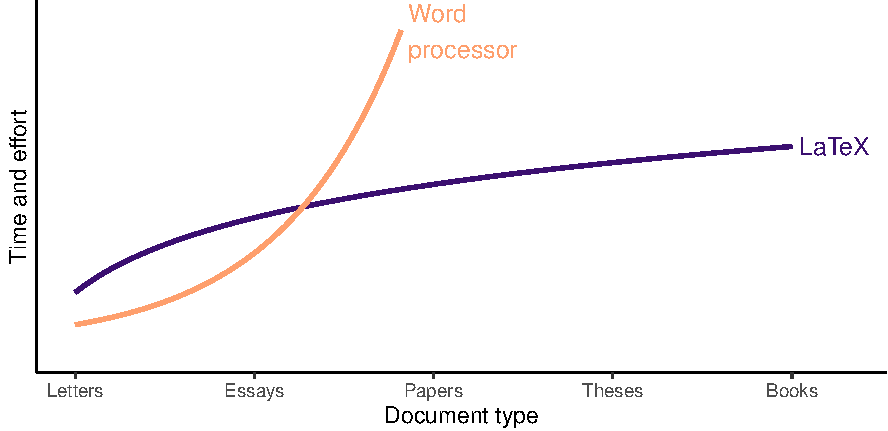
\includegraphics{figure/latexgraph-1} \end{center}
\end{frame}

\begin{frame}{Things that it solves: Picture alignment/placement}
\protect\hypertarget{things-that-it-solves-picture-alignmentplacement}{}
\LaTeX~takes care of figure placements automatically.

\begin{columns}[T]
\begin{column}{0.64\textwidth}
\begin{center}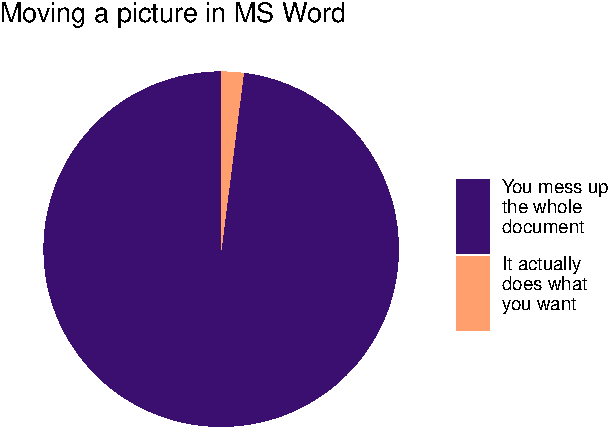
\includegraphics{figure/piechart-1} \end{center}
\end{column}

\begin{column}{0.33\textwidth}
\vspace{2em}

\begin{figure}
\frame{
\includegraphics[width=\linewidth]{figure/tweet_msword.pdf}}
\end{figure}
\end{column}
\end{columns}
\end{frame}

\begin{frame}{Things that it solves: References and bibliography}
\protect\hypertarget{things-that-it-solves-references-and-bibliography}{}
Sometimes, however, what others tell us is important as
\emph{corroboration} of what we have already found out (or think we have
found out) for ourselves. The Scottish philosopher Thomas Reid makes
this point in connection with mathematical research in the belief that,
if it applies to the science `in which, of all sciences, authoritiy is
acknowledges to have least weight' \cite{reid2002thomas}, it will be
even more significant in other areas of thought and practice\ldots{}
Russell, as we shall see in a later chapter, considered this aspect of
our reliance upon testimony essential to the understanding of what it is
to be a physical thing and he criticized logical positivism for its
failure to appreciate the implications of this point
\cite{russell2007logic}. In the Analysis of Matter he says explicitly,
`I mean here by ``objective'' not anything metaphysical but merely
``agreeing with the testimony of others''' \cite{russell2015analysis}.

\vspace{1em}

Excerpt from \emph{Testimony: A Philosophical Study} by C. A. J. Coady
(1992)
\end{frame}

\begin{frame}{References}
\protect\hypertarget{references}{}
\nocite{coady1992testimony} \printbibliography[heading=none]
\end{frame}

\begin{frame}{Things that it solves: Mathematical equations}
\protect\hypertarget{things-that-it-solves-mathematical-equations}{}
Typesetting mathematics and equation referencing.

\vspace{1em}

\hrule

\vspace{0.5em}

\begin{theorem}[Central Limit Theorem]
\label{thm:clt} Let \(X_1,\dots,X_n\) be an independent random sample
from a distribution whose mean is \(\mu\) and variance is \(\sigma^2\).
Then \(\bar X_n := \frac{1}{n}\sum_{i=1}^n X_i\) converges in
distribution to a random variable whose density function is
\begin{equation}
\label{eq:clt}
f(x) = \frac{1}{\sqrt{2\pi}} \exp\left[ -\frac{1}{2}\left(\frac{x - \mu}{\sigma/\sqrt n} \right)^2 \right]
\end{equation}
\end{theorem}

The proof of Theorem \ref{thm:clt} uses \emph{charactertistic
functions}, whereby the standardised version of \eqref{eq:clt} is
obtained in the limit.
\end{frame}

\begin{frame}{A chemistry example}
\protect\hypertarget{a-chemistry-example}{}
\begin{figure}
    \centering
    \small
    \schemestart
        \chemname{
            \chemfig{
                CH
                (-[:90]CH_2-OOC-R_1)
                (-[:-90]CH_2-OOC-R_3)
                -OOC-R_2
            }
        }{Triglyceride}
        \+
        \chemname{
                \chemfig{
                    3 ROH
                }
            }{Alcohol}
        \arrow(.mid east--.mid west){<=>[Catalyst]}
        \chemname{
            \chemfig{
                R_2
                (-[:90,,,,draw=none]R_1-COO-R)
                (-[:-90,,,,draw=none]R_3-COO-R)
                -COO-R
            }
        }{Alkyl esters}
        \+
        \chemname{
            \chemfig{
                CH
                (-[:90]CH_2-OH)
                (-[:-90]CH_2-OH)
                -OH
            }
        }{Glycerol}
    \schemestop
    \caption{Transesterification of triglyceride with alcohol.}
    \label{scm:tsester}
\end{figure}

\blfootnote{Figure \ref{scm:tsester} obtained from \url{https://tex.stackexchange.com/a/472486}}
\end{frame}

\begin{frame}{Languages}
\protect\hypertarget{languages}{}
\vspace{-2em}

\begin{columns}[T]
\begin{column}{0.48\textwidth}
\begin{center}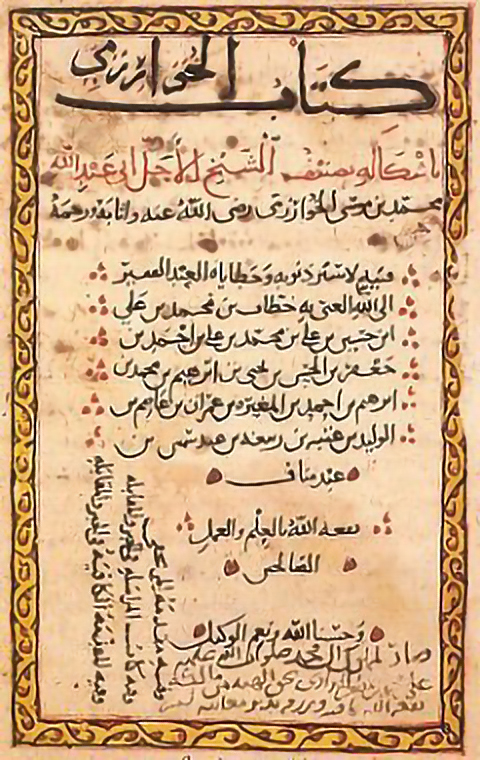
\includegraphics[width=0.4\linewidth]{figure/00-aljabr} \end{center}

\textarabic{
الْكِتَابْ الْمُخْتَصَرْ فِيْ حِسَابْ الْجَبْرْ وَالْمُقَابَلَة
} (The Compendious Book on Calculation by Completion and Balancing),
also known as \textarabic{الجبر} (Al-Jabr), written by \textarabic{
محمد بن موسى الخوارزميّ
} (Muḥammad ibn Mūsā al-Khwārizmī) around 820 CE.
\end{column}

\begin{column}{0.48\textwidth}
\begin{center}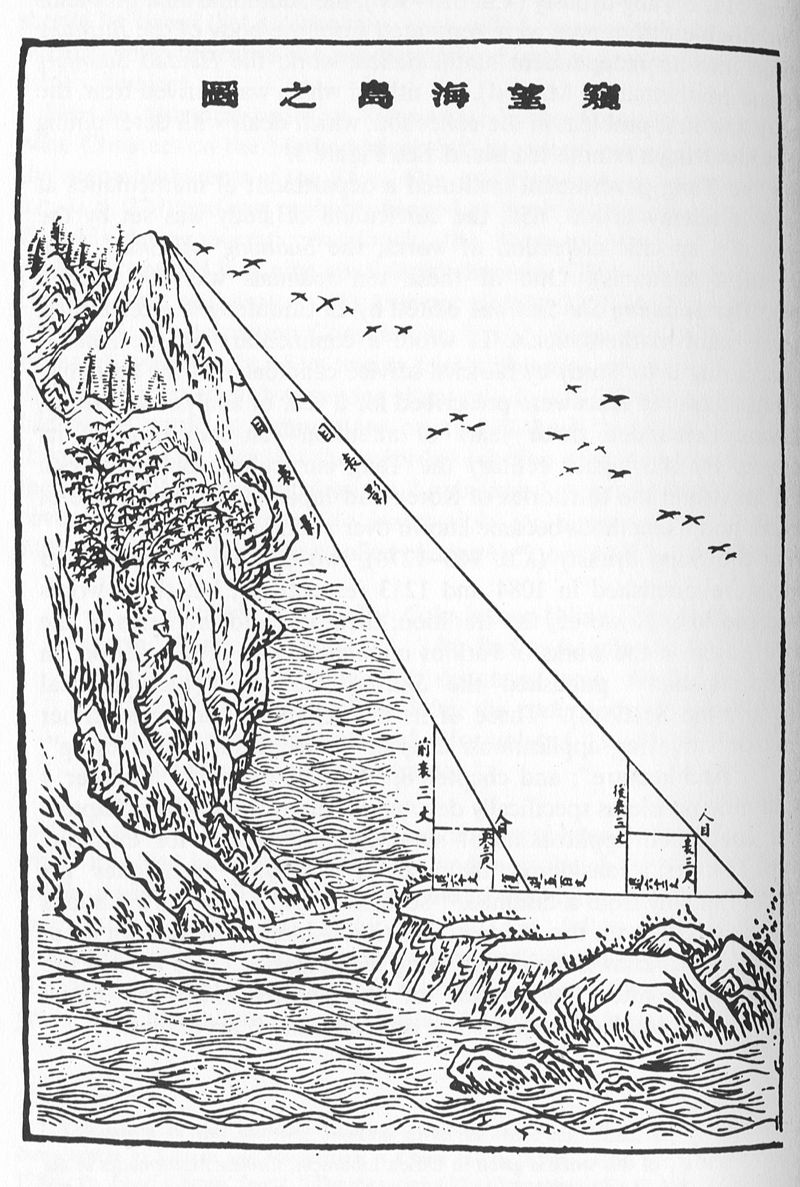
\includegraphics[width=0.4\linewidth]{figure/00-haidaosuanjing} \end{center}

海岛算经 (Hǎidǎo suàn jīng--The Sea Island Mathematical Manual) was
written by 刘徽 (Liú Huī) ca. 200 CE. The Chinese were aware of a good
approximation of \(\pi\approx\) \(355/113\) \(= 3.1415929204\) very
early on (祖冲之 Zǔ Chōng Zhī, 500 CE).
\end{column}
\end{columns}
\end{frame}

\begin{frame}{For teaching}
\protect\hypertarget{for-teaching}{}
\begin{itemize}
\tightlist
\item
  Setting of question papers (assignments, tests, exams, etc.)
\item
  Syllabus documents
\item
  Presentations
\end{itemize}
\end{frame}

\hypertarget{getting-started}{%
\section{Getting started}\label{getting-started}}

\begin{frame}[fragile]{Getting started}
\protect\hypertarget{getting-started-1}{}
\framesubtitle{A minimal \LaTeX\ document}

\begin{Shaded}
\begin{Highlighting}[]
\BuiltInTok{\textbackslash{}documentclass}\NormalTok{\{}\ExtensionTok{article}\NormalTok{\}}
\KeywordTok{\textbackslash{}begin}\NormalTok{\{}\ExtensionTok{document}\NormalTok{\}}
\NormalTok{Hello, World!  }\CommentTok{\% your content goes here...}
\KeywordTok{\textbackslash{}end}\NormalTok{\{}\ExtensionTok{document}\NormalTok{\}}
\end{Highlighting}
\end{Shaded}

\begin{itemize}
\item
  Commands start with a backslash \texttt{\textbackslash{}}
\item
  Every document starts with a \texttt{\textbackslash{}documentclass}
  command
\item
  The \emph{argument} in curly braces \texttt{\{} \texttt{\}} tells
  \LaTeX~what kind of document we are creating (in this case, an
  \texttt{article})
\item
  A percent sign \texttt{\%} starts a \emph{comment}--\LaTeX~will ignore
  the rest of the line
\end{itemize}
\end{frame}

\begin{frame}{Getting started}
\protect\hypertarget{getting-started-2}{}
\framesubtitle{Overleaf}

\begin{columns}[T]
\begin{column}{0.3\textwidth}
\centering
\vspace{-2em}

\begin{center}
\includegraphics[width=0.9\linewidth]{figure/overleaf} \end{center}

\vspace{-1em}

\url{https://www.overleaf.com/}
\end{column}

\begin{column}{0.68\textwidth}
\begin{varblock}{Exercise 1}
1

\end{varblock}
\end{column}
\end{columns}

\vspace{1em}

\begin{itemize}
\item
  Overleaf is a website for writing documents in \LaTeX
\item
  It `compiles' your \LaTeX~document online to show you the results
\item
  As we go through the following slides, try out the examples by typing
  them into the example document on Overleaf!
\end{itemize}

\begin{alertblock}{Reminder}
Sign up for Overleaf

\end{alertblock}
\end{frame}

\begin{frame}{Exercises}
\protect\hypertarget{exercises}{}
\end{frame}

\hypertarget{mathematics}{%
\section{Mathematics}\label{mathematics}}

\hypertarget{figures-and-others}{%
\section{Figures and others}\label{figures-and-others}}

\hypertarget{document-structure}{%
\section{Document structure}\label{document-structure}}

\hypertarget{bibliography}{%
\section{Bibliography}\label{bibliography}}




\end{document}		